\chapterimage{/7/head.jpg} % Chapter heading image
\chapter{Un'oscillazione non è per sempre}\label{7:ch}

\subsection{Hot N Cold Dark Matter}
Da un punto di vista cosmologico, l'interesse principale non è nella/e particella/e costituenti la materia oscura, ma nei suoi effetti. In particolare deve interagire debolmente con la materia barionica e con sé stessa (da cui la categoria delle \textit{Weakly Interacting Massive Particles}). Data una nuova particalla teorizzata, e.g. il \textit{laurino}, i cosmologi vorrebbero sapere:
\begin{enumerate}
    \item Massa: definisce a grandi linee il momento in cui la particella smette di essere relativistica, dall'uguaglianza $k_B T = m_xc^2$. Le particelle che smettono di essere relativistiche più tardi sono quelle via via più leggere.
    \item Interazione con fluido radiativo e altre particelle: definisce il tempo di disaccoppiamento con le altre componenti $\tau = (n_x c \sigma)^{-1}$.
\end{enumerate}

Si definiscono particelle di \textbf{materia oscura calda (HDM)} quelle ancora relativistiche al momento del disaccoppiamento dal fluido: $\tau_{dec,x}<\tau_{nRel}$. Tipico candidato è il neutrino, con la sua massa estremamente piccola. Quelle per cui vale la relazione inversa sono particelle di \textbf{materia oscura fredda (CDM)}. Vanno quindi confrontati tre tempi fondamentali: $\tau_{dec,x}$, $\tau_{nRel}$, $\tau_{eq}$. 
Come si è visto il disaccoppiamento delle particelle di materia oscura avviene nell'era radiativa. La massa di una particella che diventa non relativistica a $t_{eq}$ è:
$$
z_{eq}\simeq 10^4; \quad T_{eq}\simeq 3\cdot 10^4 \: K \quad \rightarrow \quad m_x\simeq 1\: eV
$$
Tutte le particelle con massa più grande di $1\: eV$ (sostanzialmente tutte a parte il neutrino, $m_\nu\simeq few\:\cdot 0.1\: eV$) si sono già de-relativizzate prima dell'equivalenza.

\vspace{1em}

La differenza tra HDM e CDM è da ricercarsi nel fatto che la scala di Jeans dipende dalla velocità della particella e la HDM era ancora relativistica al momento del disaccoppiamento. Per ambedue, il massimo della scala di Jeans è raggiunto al momento dell'equivalenza e vale:
\begin{equation}\left.
    \def\arraystretch{1.3}
        \begin{array}{llll}
        HDM & M_J (t_{eq}) \simeq 10^{15} M_\odot\\
        CDM & M_J (t_{eq})\lesssim 10^{5\div 6} M_\odot
    \end{array}\right.
\end{equation}

Una perturbazione su scala maggiore di $M_J$ può crescere, in particolare tutte le scale maggiori di $M_J(t_{eq})$ crescono sempre. Viceversa, le scale minori, crescono oscillano e \stkout[.5pt]{ricrescono} vengono cancellate (paragrafo successivo). Ovviamente questo discorso ha senso entro l'orizzonte, fuori le perturbazioni crescono sempre. I calcoli della massa di Jeans nei tre (quattro per la CDM) tempi fontamentali sono riportati nella Sezione \ref{ch7:complementi}, gli andamenti sono illustrati nella Figura \ref{fig7:mjhotncold}.

\begin{figure}[H]
    \centering
    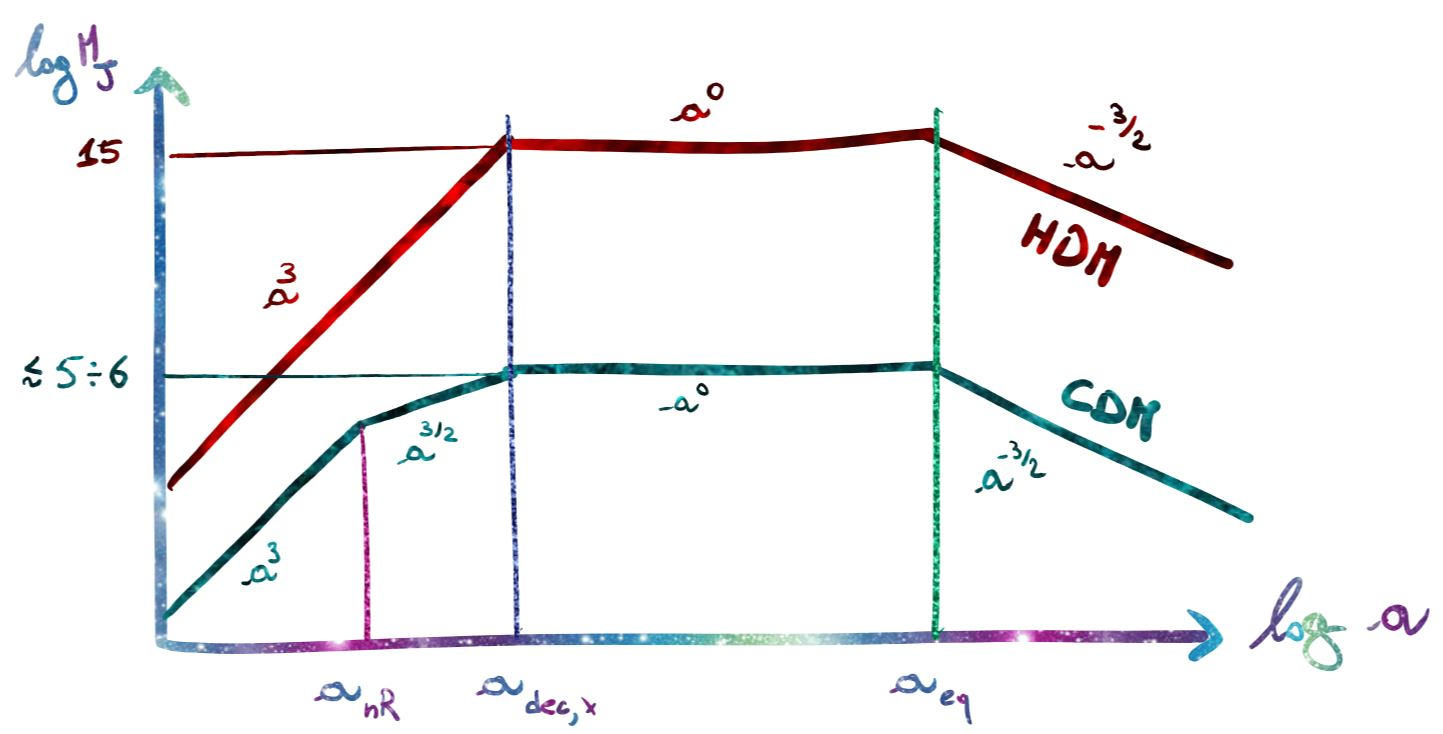
\includegraphics[width=.88 \textwidth]{Pictures/7/mjhotncold.jpg}
    \caption{Evoluzione della massa di Jeans per HDM e CDM al variare del parametro di espansione (tempo).}\label{fig7:mjhotncold}
\end{figure}

\subsection{Massa di Jeans dei barioni}
Viene definito un redshift equivalente a $z_{eq}$, ma per soli barioni: $z_{eq,b}: \; \rho_b=\rho_r$, inserendo la rispettiva dipendenza della densità dal redshift si ottiene:
\begin{equation}
    1+z_{eq,b}=\frac{\Omegabo}{\Omegaro}\simeq 3.9\cdot 10^4\; \Omegabo h^2
\end{equation}

Il disaccoppiamento avviene dopo aver raggiunto l'equivalenza in densità barionica ($z_{dec,b}<z_{eq,b}$) soltando per valori di $\Omegabo h^2 > 0.028$. Planck ha misurato $\Omegabo h^2 = 0.022$. Dato che il valore discriminante è molto vicino a quello misurato, si considereranno entrambi i casi. Gli andamenti nei diversi periodi in esame sono calcolati nella Sezione \ref{ch7:complementi} e illustrati nella Figura \ref{fig:7mjbar}. Si ricorda che sono in esame perturbazioni di tipo adiabatico. Il massimo della scala di Jeans è raggiunto al momento dell'equivalenza/disaccoppiamento e vale:
\begin{equation}\left.
    \def\arraystretch{1.3}
        \begin{array}{l}
     M_{J,b} (t_{dec}) \simeq 10^{16} M_\odot\\
    \end{array}\right.
\end{equation}
\begin{figure}[H]
    \centering
    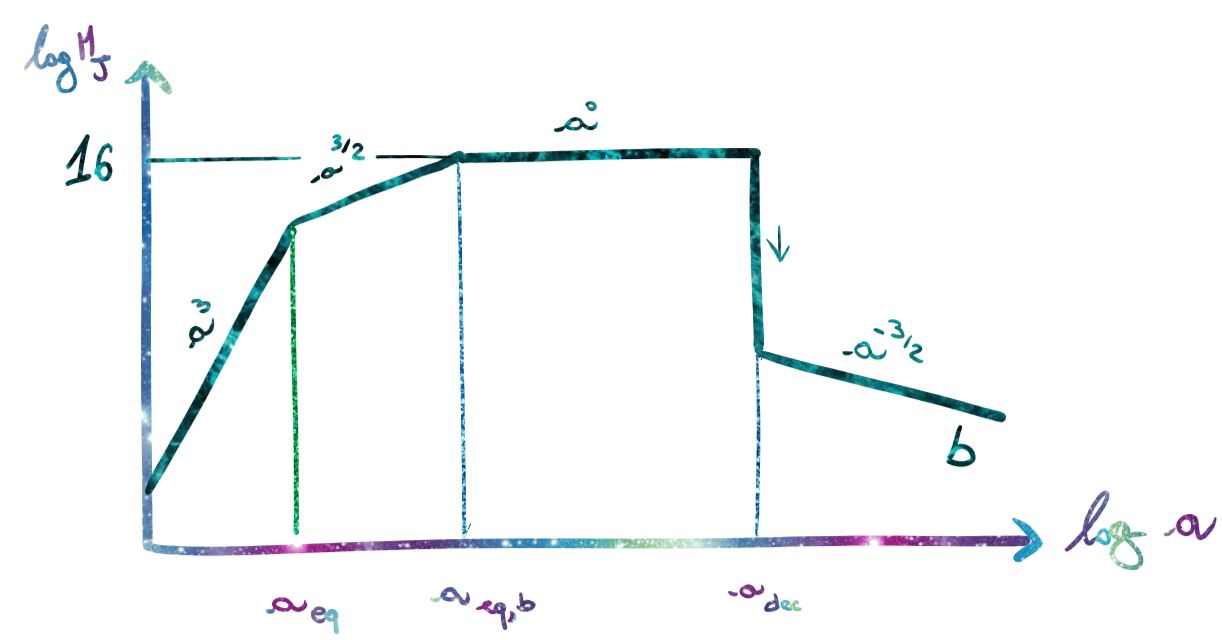
\includegraphics[width=.9 \textwidth]{Pictures/7/mjbar.jpg}
    \caption{Il salto nella normalizzazione è dovuto al fatto che viene a mancare il supporto della radiazione.}\label{fig:7mjbar}
\end{figure}

\section{Materia oscura e \textit{free streaming}}
La particella di materia oscura classica non è collisionale. Per questo motivo di parla di \textit{free streaming} e non di dissipazione. Le particelle, di fatto, rispondono al potenziale medio (quello dell'universo omogeneo), il quale tende a ri-livellare i contrasti di densità. Si definisce \textbf{scala di free-streaming}:
$$
\lambda_{fs}(t) = a(t)\int_0^t \frac{v_{DM}(t')\d{t'}}{a(t')}
$$

Gli andamenti risultanti sono calcolati nella Sezione \ref{ch7:complementi}, inoltre l'evoluzione di $M_{fs}$ è confrontata con $M_J$ nella Figura \ref{fig:7mfscold}. Stando a quanto visto, sotto la scala di Jeans le onde di densità si propagano, ciononostante le scale via via raggiunte da $\lambda_{fs}$ vengono cancellate.

\begin{figure}[H]
    \centering
    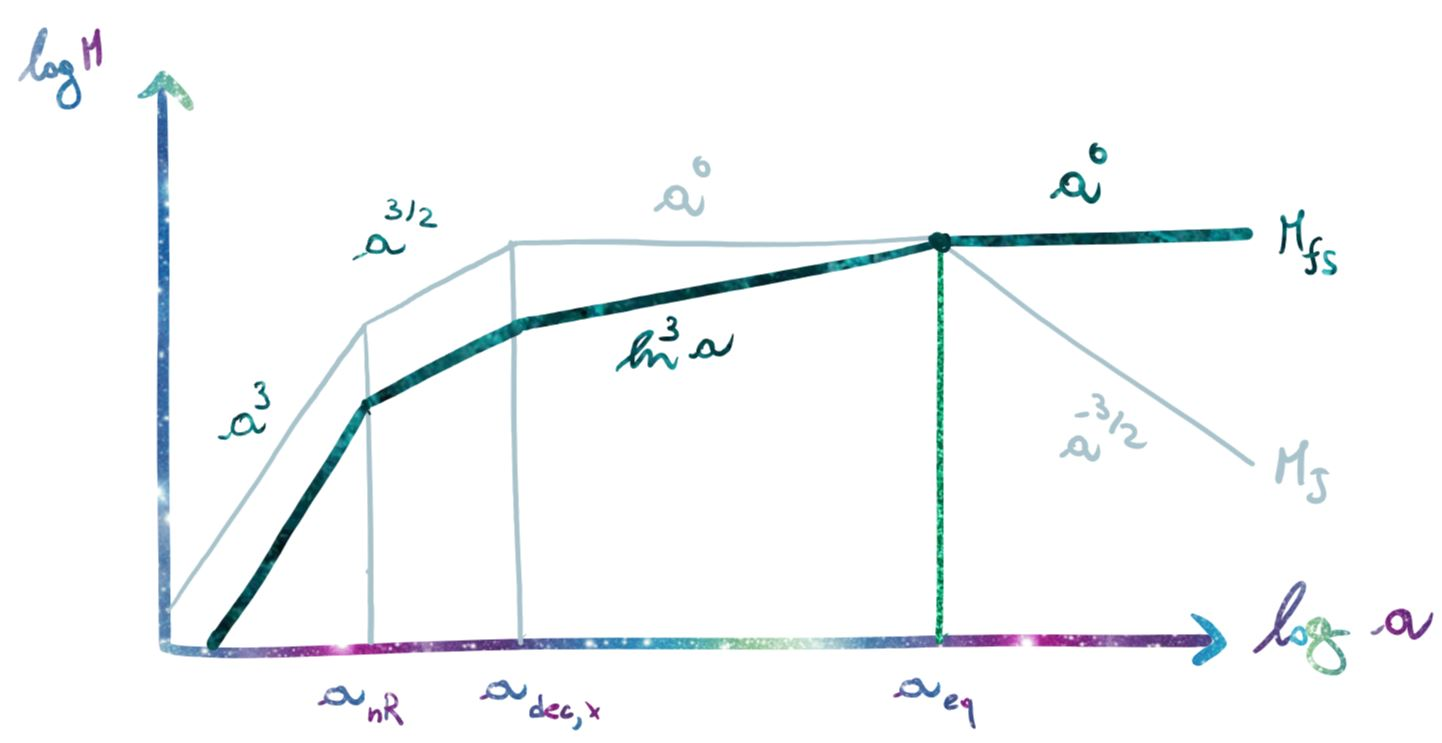
\includegraphics[width=.9 \textwidth]{Pictures/7/mfscold.jpg}
    \caption{Evoluzione di $M_{fs}$ confrontata con $M_J$ normalizzate in $a_{eq}$, si può dimostrare matematicamente che $M_J(t_{eq})=M_{fs}(t_{eq})$. Per definizione la $M_{fs}$ (come il raggio dell'orizzonte) non può decrescere, al massimo rimane costante.}\label{fig:7mfscold}
\end{figure}

\begin{theorem}[Messaggio da portare a casa]
 Dall'equivalenza in poi sopravvivono soltanto le perturbazioni su scala $>M_J$ e poiché $M_J(t_{eq})=M_{fs}(t_{eq})=cost\;\; \forall t>t_{eq}$, tutte le perturbazioni su scale minori non oscillano, vengono \textbf{cancellate}.
\end{theorem}

\vspace{1em}
Nel caso della HDM si ha $M_J(t_{eq})\sim 10^{16}M_\odot$, per cui strutture più piccole (come galassie, ammassi globulari e cose di questo tipo) si devono essere per forza formate per frammentazione di megapalle. Questo scenario è detto \textbf{top-down} (o modello antigerarchico) e prevede che le strutture più grandi siano più vecchie di quelle piccole. Lo scenario alternativo, che ora va per la maggiore, è il \textbf{bottom-up} (o modello gerarchico). Esso richiede particelle di materia oscura fredda e prevede, al variare della loro massa, un valore di $M_J(t_{eq})\sim 1\div 10^{6}M_\odot$. In questo caso si formano prima le strutture piccole, poi per merging gravitazionale quelle più grandi. 

Osservando gli aloni di materia oscura si ha evidenza che questi sono più giovani delle galassie, in accordo col modello gerarchico degli aloni. Quello che succede dentro le galassie è più complesso perché entra in gioco la microfisica del gas (si osserva un comportamento antigerarchico, Thomas et al. 2005)

\newpage
\section{Materia barionica e dissipazione}
In questo caso, e solo in questo caso, si può parlare di scala di dissipazione. In particolare, ci sono due processi che riguardano i barioni: 
\begin{enumerate}
    \item Il libero cammino medio del fotone che si porta dietro il barione $\propto 1/n$ (tende a cancellare le perturbazioni su scale più piccole di $\lambda_{mfp}$);
    \item Lo scattering di fotoni che tende a far perdere coerenza alle onde di perturbazione (dissipazione per urti), come il cammino di un ubriaco.
\end{enumerate}
Il primo è più efficiente perché si oppone alla gravità, il secondo è casuale (?). La scala più grande sotto la quale viene cancellata la perturbazione è:
\begin{equation*}
   \d{x^2} = N_{urti}\lambda_{mfp}^2 = \frac{c\: \d{t}}{\lambda_{mfp}}\lambda_{mfp}^2  = c\: \lambda_{mfp}(t)\d{t}; \qquad \lambda_{mfp}(t)\propto (\sigma_T\rho_b)^{-1}\propto a^{3}
\end{equation*}

Sostituendo i dovuti andamenti di $a$ col tempo e introducendo come massa-scala la cosiddetta \textbf{massa di Silk} si ha:
\begin{equation}x \propto a^\beta \qquad \beta=\left\{
    \def\arraystretch{1.5}
        \begin{array}{llll}
        5/2 & a<a_{eq} & \rightarrow & M_{Silk}\propto a^{9/2} \\
        9/4 & a>a_{eq} & \rightarrow & M_{Silk}\propto a^{15/4}
    \end{array}\right.
\end{equation}

Dopo il disaccoppiamento il libero cammino medio è infinito e non si dissipa più nulla. In questo caso gli andamenti sono diversi da quelli della scala di Jeans, inoltre si ha 
\begin{equation}
    M_{Silk}(t_{dec})\simeq 10^{12}M_\odot
\end{equation}

Per cui, a differenza della materia oscura, la dissipazione non avviene per tutte le scale sotto a $M_J(t_{dec})$, ma esiste un intervallo di scale $\sim 10^{12}\div 10^{16}M_\odot$ in cui le oscillazioni non vengono cancellate e riscrescono dopo $t_{dec}$. Lo spettro delle perturbazioni viene modificato in maniera diversa in funzione della scala (Fig. \ref{fig:7msilkbar}). 
\begin{figure}[H]
    \centering
    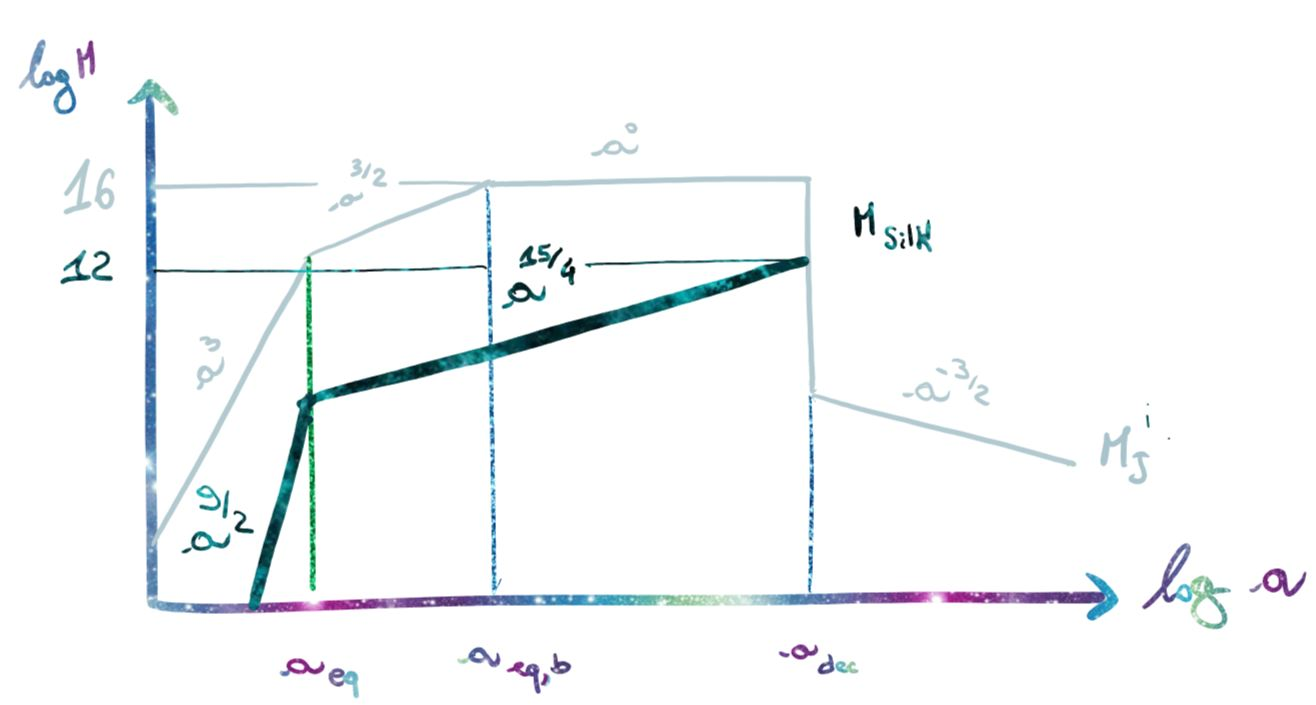
\includegraphics[width=.95 \textwidth]{Pictures/7/msilkbar.jpg}
    \caption{Evoluzione di $M_{fs}$ confrontata con $M_J$ con le dovute normalizzazioni. Per definizione la $M_{Silk}$ (come il raggio dell'orizzonte) non può decrescere, al massimo rimane costante.}\label{fig:7msilkbar}
\end{figure}



\newpage
\section{Complemento: Scale di Jeans, \textit{free streaming} e dissipazione}\label{ch7:complementi}

Per ottenere gli andamenti dalla scala di Jeans e di \textit{free streaming} della \textbf{materia oscura} è necessario ricordare:
\begin{itemize}
    \item $\lambda_J = v_{part}/\sqrt{G\rho}$
    \item $\rho$ è quella della componente dominante ($\propto a^{-4}$ prima di $t_{eq}$ e $\propto a^{-3}$ dopo)
    \item Dalla teoria di Jeans cosmologica $v\propto a^{-1}$ nel caso di moto libero senza processi dissipativi
    \item $M_J\propto \lambda_J^3 a^{-3}$
    \item La definizione di $\lambda_{fs}$
\end{itemize}

\begin{equation}\left.
    \def\arraystretch{1.5}
        \begin{array}{c|llllll}
         & v^2 & \lambda_{J,DM} & M_{J,DM} & \lambda_{fs}& M_{fs} & \\ \midrule
        a < a_{nRel} & c^2/3 & \propto a^2  & \propto a^3 & \propto a^2 & \propto a^3  & \\
        a_{nRel}< a < a_{dec,x} & \propto a^{-1} & \propto a^{3/2} &  a^{3/2} & \propto a^{3/2} & \propto a^{3/2} & (CDM) \\
        a_{dec,x}< a < a_{eq} & \propto a^{-2}  & \propto a & cost & \propto a\ln a & \propto \ln^3 a& \\
        a > a_{eq} & \propto a^{-2} & \propto a^{1/2} &  a^{-3/2} &\propto a  & cost &
    \end{array}\right. \label{tab:7jfsdm}
\end{equation}

\vspace{2em}
Per ottenere le dipendenze dalla scala di Jeans e della \textbf{materia barionica} è necessario ricordare:
\begin{itemize}
    \item I punti ricordati 15 cm fa
    \item $c_s^2=p/\rho$
    \item Per $a_{eq}$ si intende ovviamente $a_{eq,DM}$
\end{itemize}
\begin{equation}\left.
    \def\arraystretch{1.5}
        \begin{array}{c|lllll}
             & c_s^2 & \lambda_{J,b} & M_{J,b} & M_{Silk} & \\ \midrule
        a<a_{eq} & cost & \propto a^2 & \propto a^3 & \propto a^{9/2} &\\
        a_{eq} < a<a_{eq,b} & cost &  \propto a^{3/2} & \propto a^{3/2} & \propto a^{15/4} & \\
        a_{eq,b} < a < a_{dec,b} & \propto a^{_1} & \propto a & cost & \propto a^{15/4} & (se\; esiste) \\
        a > a_{dec,b} & \propto a^{-2} & \propto a^{1/2} & \propto a^{-3/2} & &
    \end{array}\right.  \label{tab:7jbar}
\end{equation}